\documentclass[graphics]{beamer}

\usepackage{graphicx}
\usepackage{verbatim}
\usepackage{wrapfig}
\useoutertheme{shadow}
%\usecolortheme{orchid}
\usecolortheme{seahorse}


% math commands
\newcommand{\be}{\begin{eqnarray}}
\newcommand{\ee}{\end{eqnarray}}
\newcommand{\beq}{\begin{equation}}
\newcommand{\eeq}{\end{equation}}
\def\simless{\mathbin{\lower 3pt\hbox
      {$\rlap{\raise 5pt\hbox{$\char'074$}}\mathchar"7218$}}}
\def\simgreat{\mathbin{\lower 3pt\hbox
      {$\rlap{\raise 5pt\hbox{$\char'076$}}\mathchar"7218$}}} %> or of order

% variables

\def\toonscale{0.45}
\def\mboxy#1{\mbox{\small #1}}


\begin{comment}
\AtBeginSection[]{
  \frame{
    \frametitle{Outline}
    \tableofcontents[currentsection]
  }
}
\end{comment}

\title{CHIME potential for IPS
}
%\subtitle{interim update}
\author[U. Pen]{Ue-Li Pen, CITA
\\[8mm] 
}
\date{December 5, 2019}


\begin{document}

%\section*{Introduction}
\section{Current results}

\begin{comment}
  \subsection{Outline}

  \frame{
    \frametitle{Outline}
    \tableofcontents
  }
\end{comment}

\frame{\maketitle}

  \frame{
    \frametitle{CHIME}
    \begin{itemize}
        \item CHIME commissioning, first FRB's, first maps
        \item 400-800 MHz
        \item daily sky cadence, exposure time 10m/cos($\delta$)
        \item daily maps at 100 $\mu$Jy RMS noise: several times deeper
          than NVSS, millions of sources
    \end{itemize}
%\vspace{-0.1in}\hspace{.3in}
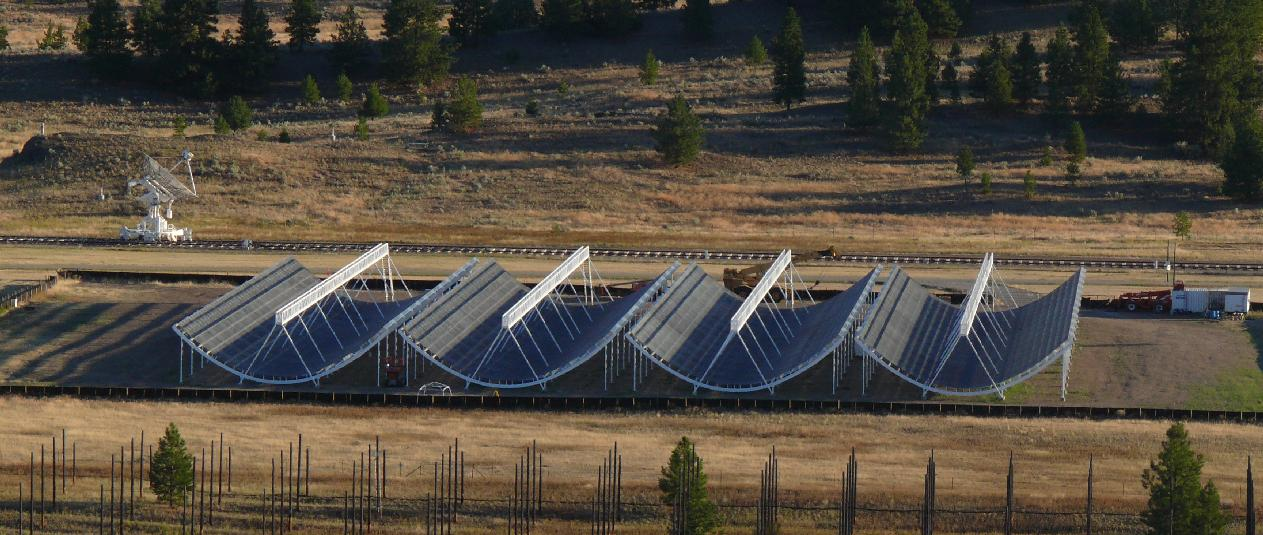
\includegraphics[width=4in]{Figures/Chime-medium.jpg}
}

  \frame{
    \frametitle{Signal flow}
%\vspace{-0.1in}\hspace{.3in}
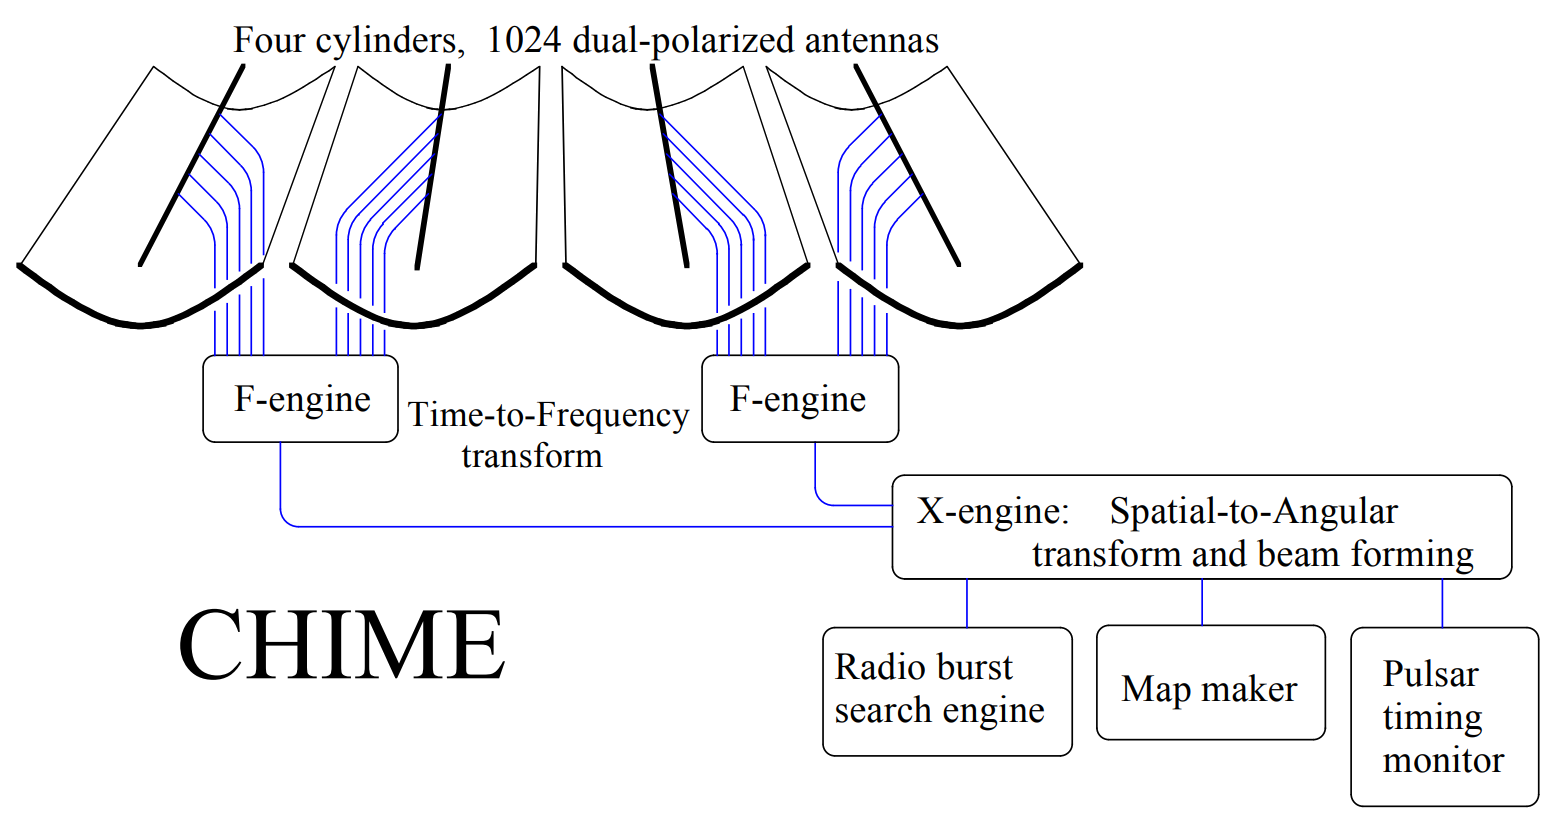
\includegraphics[width=4.5in]{Figures/instrument-figure-1.png}
}

  \frame{
    \frametitle{Beams}
%\vspace{-0.1in}\hspace{.3in}
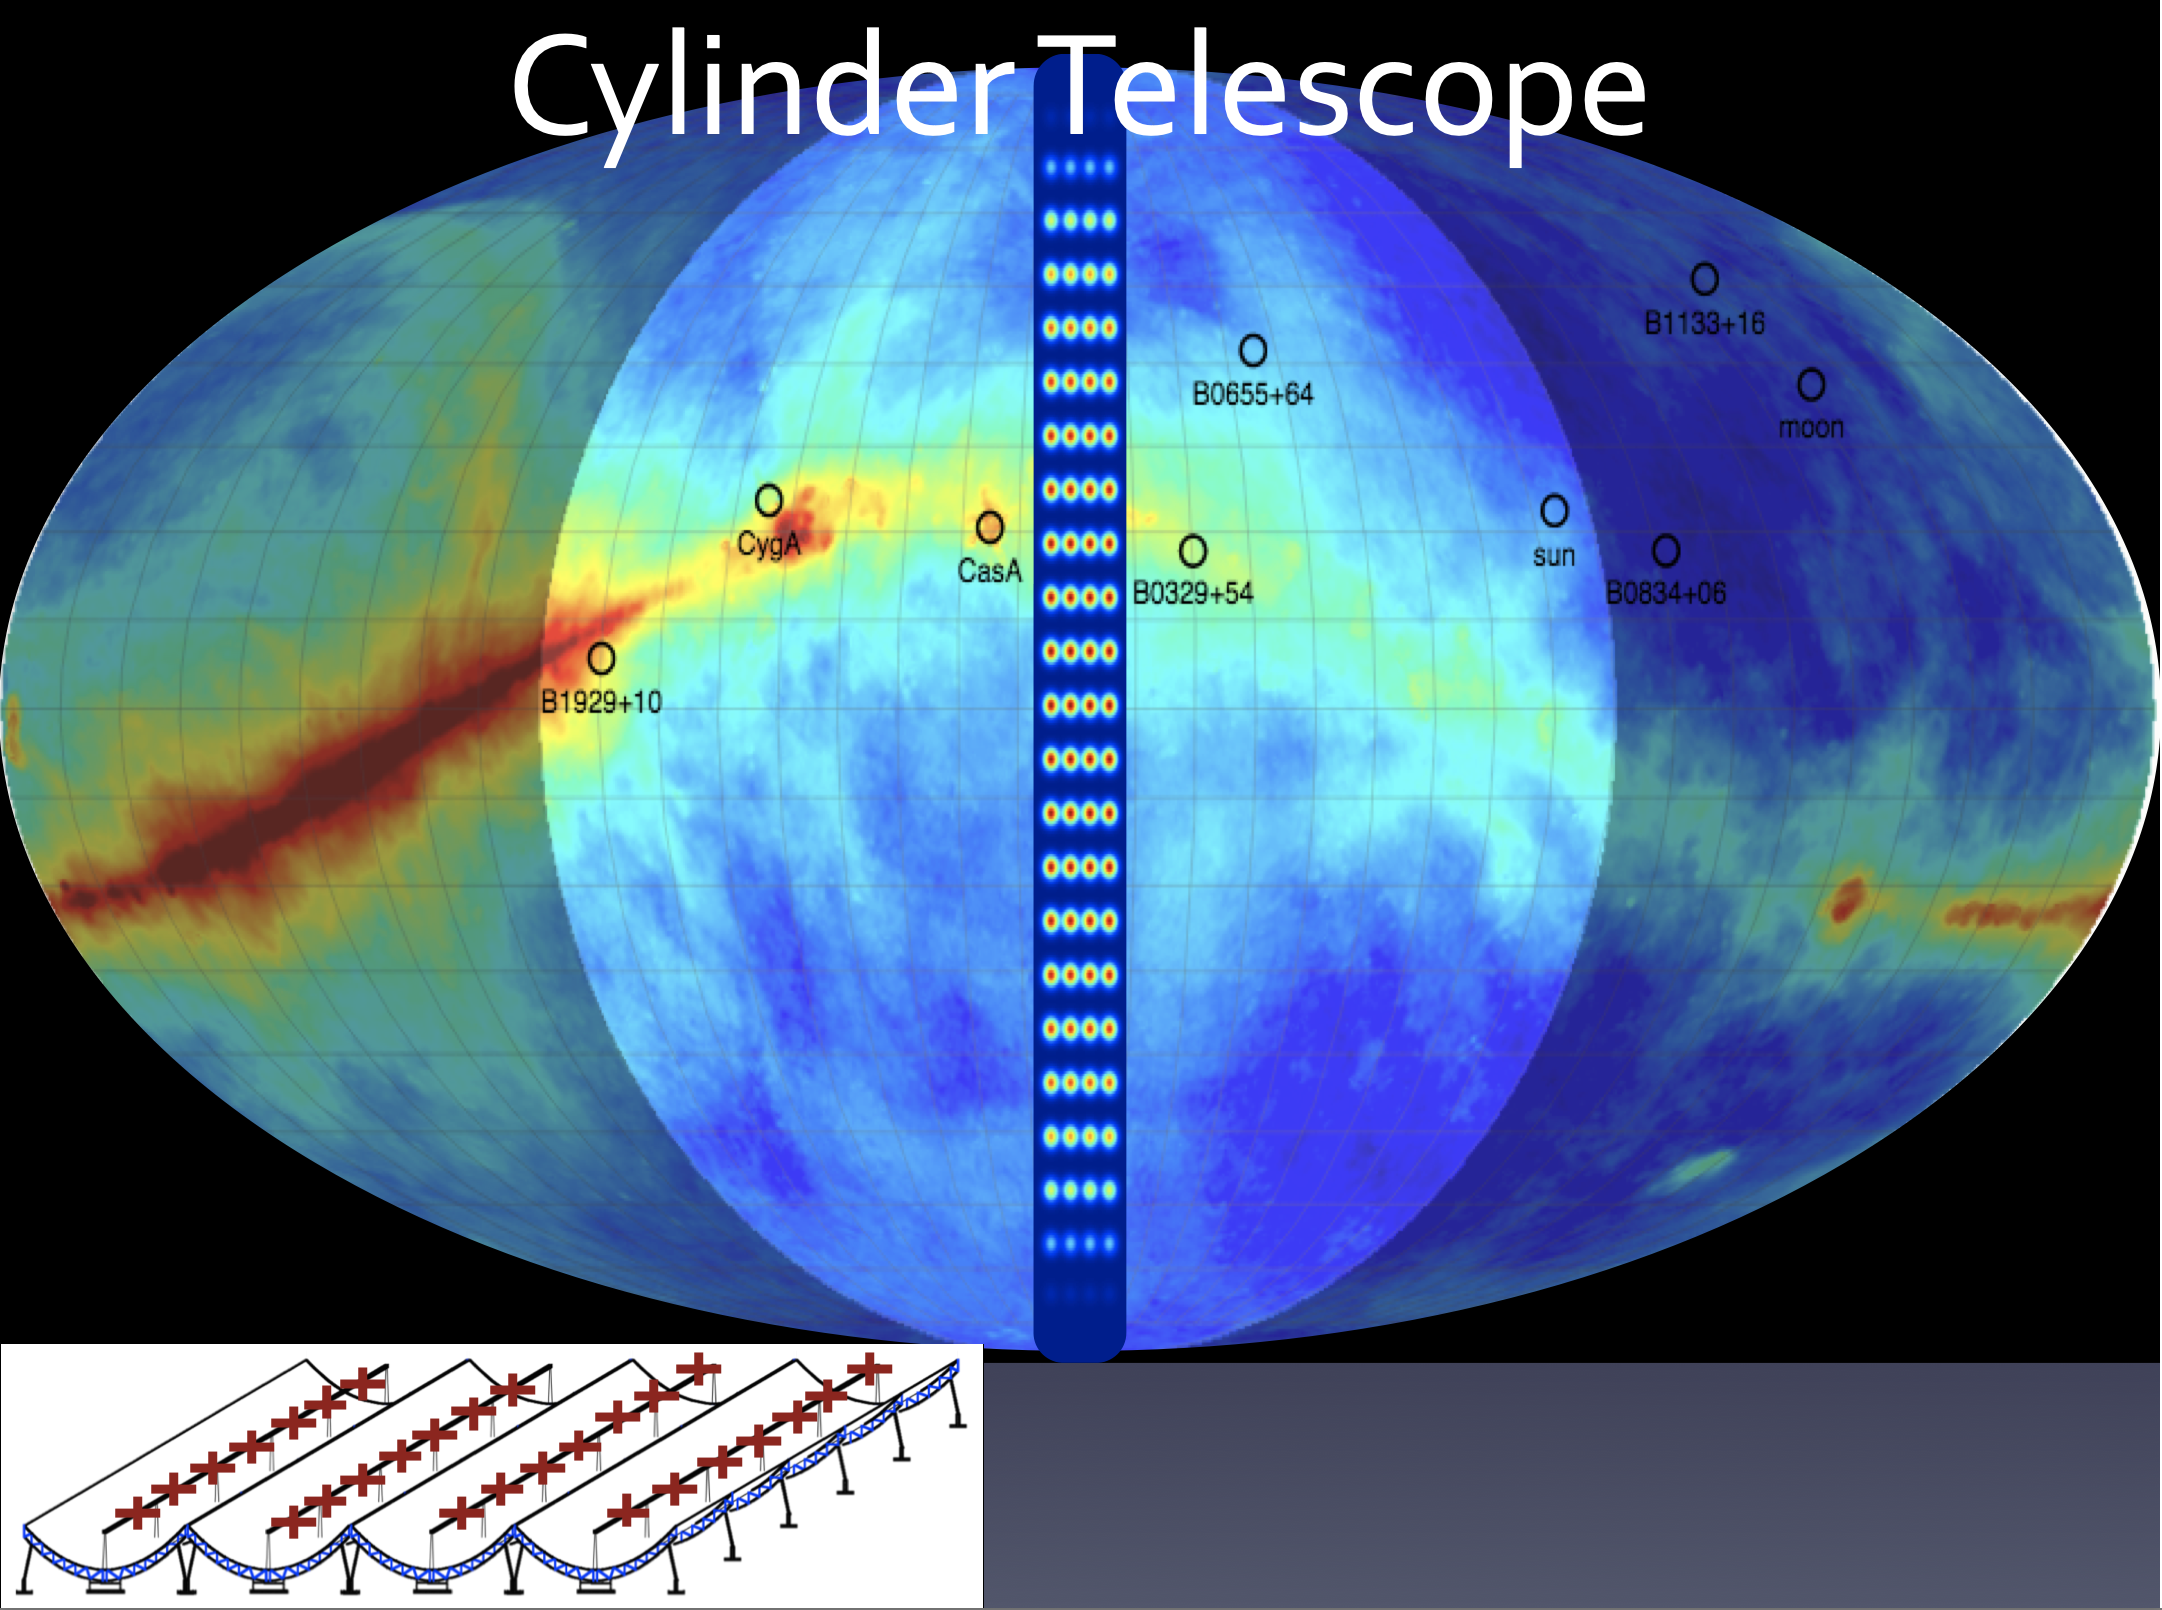
\includegraphics[width=4.1in]{Figures/liam-cylinder.png}
}


  \frame{
\vspace{-0.5in}
    \frametitle{Radio Survey Science}
    \begin{itemize}
    \item CHIME history: HSHS Paris 2006+: Peterson, Ansari, Torchinski, Pittsburgh prototype++
        \item 21cm: Intensity Mapping (Chang 2008++) BAO-DE, absorbers
        \item FRB
        \item pulsar search
        \item transients: TDE, etc
        \item polarization
        \item IPS?
    \end{itemize}
  }


  \frame{
\vspace{-0.5in}
    \frametitle{Metrics}
    \begin{itemize}
        \item flux limited survey speed: A$\Omega$
        \item time resolution: nano-sec (targeted), ms (survey)
        \item spectral resolution R=$\lambda/\Delta \lambda$: CHIME
          $\sim 10^{5-6}$
        \item dynamic range: CHIME spectral target $10^4$.
        \item trigger latency: CHIME $\sim 30$ sec
        \item localization: current $'-^o$, with outriggers $\sim$ milli-arcsec
    \end{itemize}
  }



  \frame{
\vspace{-0.5in}
    \frametitle{CHIME backends}
    \begin{itemize}
        \item FRB: ms time, 24kHz freq resolution, fast DM transform
          not saved, ongoing
        \item Cosmology: 10sec cadence, 0.4 MHz, all vis, ongoing
        \item Pulsar search: 2ms cadence, variable spectral
          resolution $<$ MHz, data archived for $\sim$ month,
          deployment 2020
        \item Absorber search: 10s cadence, 6 kHz spectra
        \item steerable beams: 10 (out of 1024), 1 w/baseband, 1.25ns time resolution
    \end{itemize}
  }

  \frame{
\vspace{-0.5in}
    \frametitle{IPS potential}
    \begin{itemize}
        \item interface playback of pulsar search stream
        \item Pulsar search: 2ms integration, variable spectral
          resolution $<$ MHz, data archived for $\sim$ month,
          deployment 2020
        \item Absorber search: 10s cadence, 6 kHz spectra
        \item steerable beams: 10 (out of 1024), 1 w/baseband, 1.25ns time resolution
    \end{itemize}
  }

  \frame{
    \frametitle{CHIME-FRBs}
    \begin{itemize}
        \item CHIME: already hundreds of FRBs after a year, upgrade to
          precision localization with outriggers
        \item orders of magnitude faster survey speed, 
          scalable 
        \item coherent sources at cosmological distance: interference
          patterns, GW, lensing, etc
    \end{itemize}
%\vspace{-0.2in}
\hspace{-0.1in}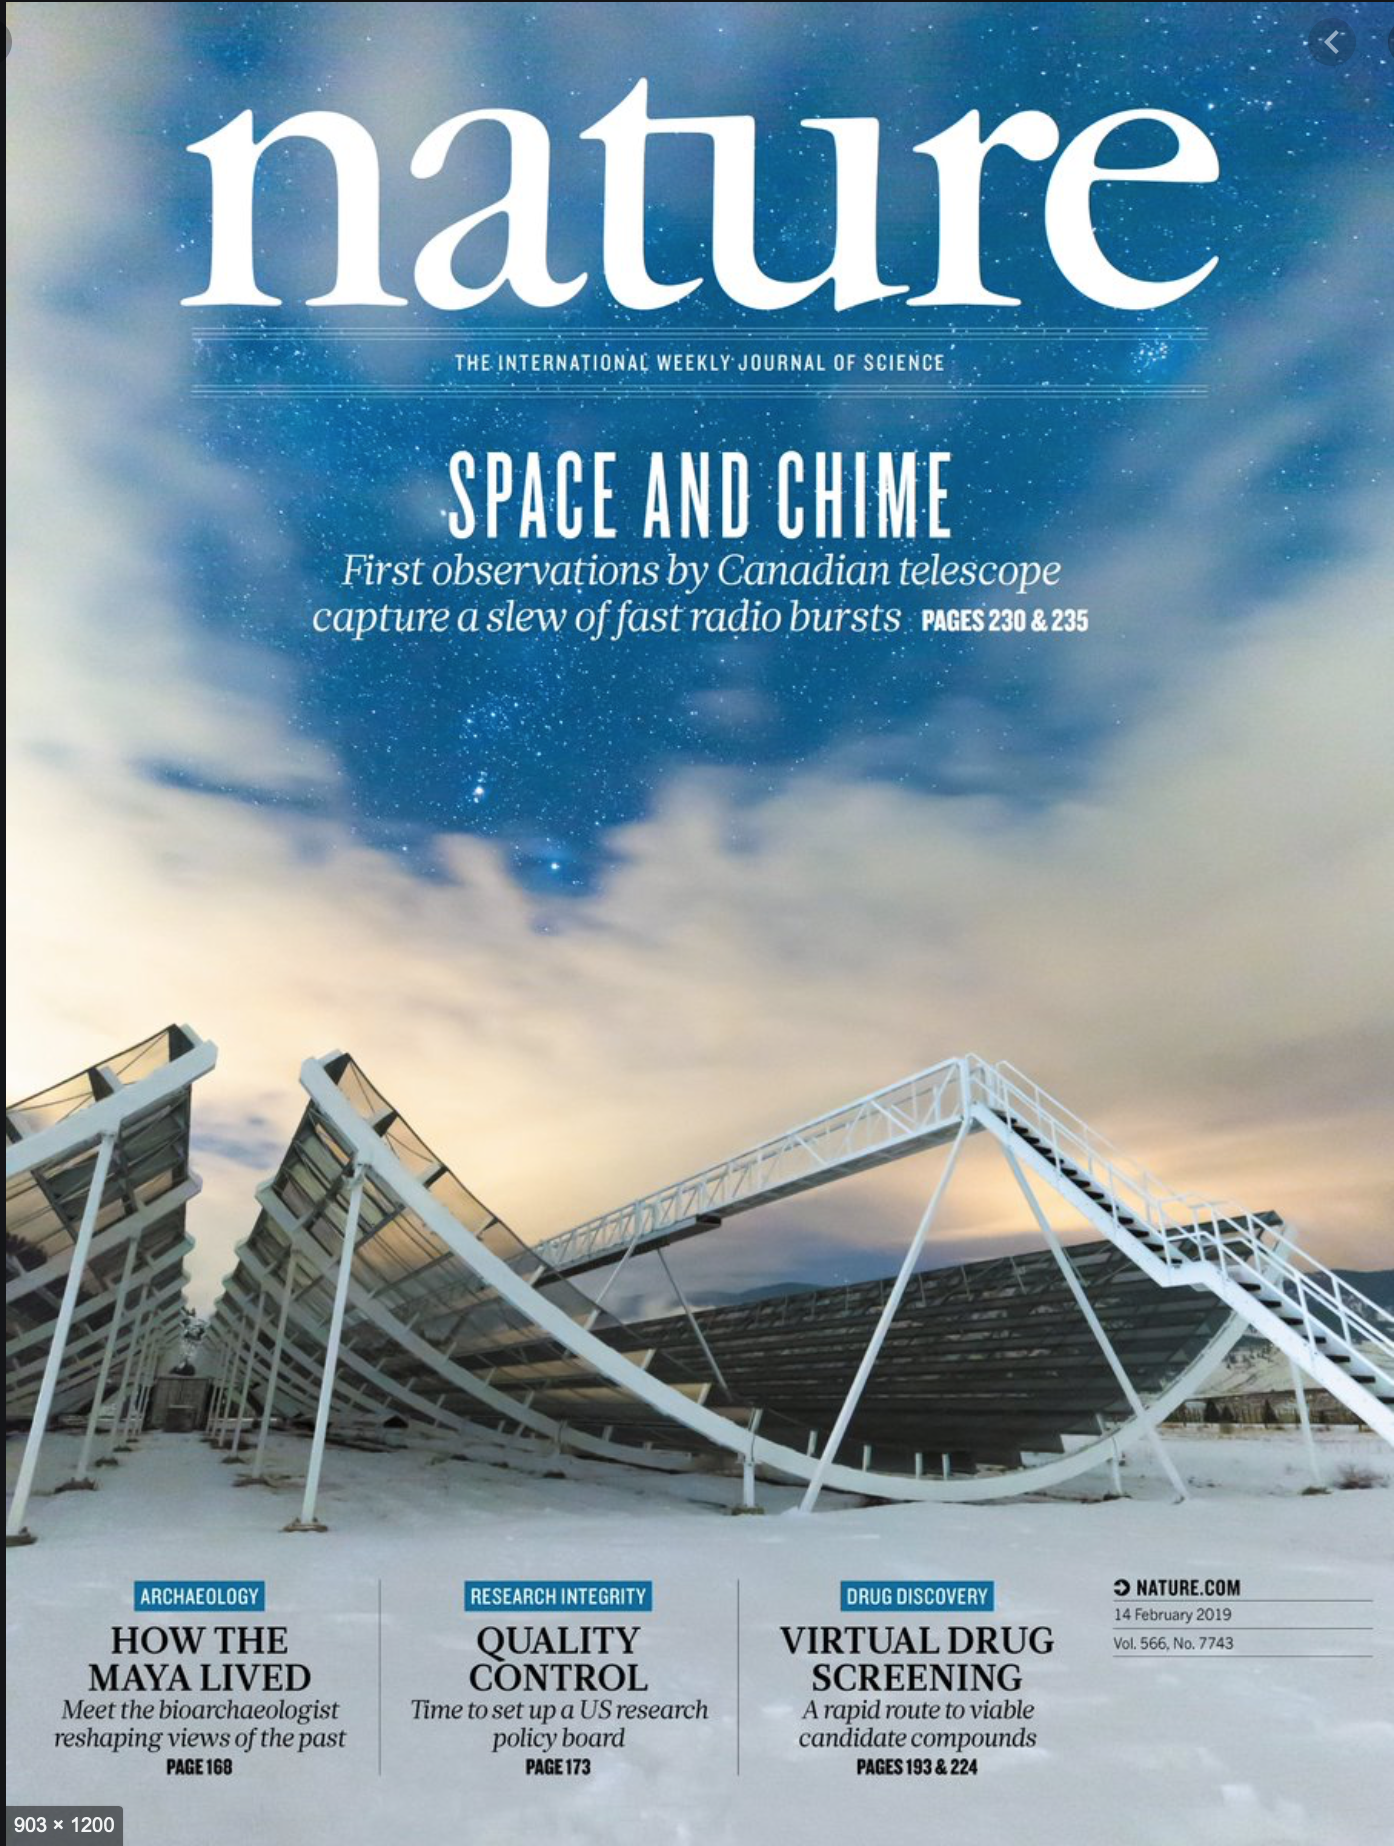
\includegraphics[width=1.6in]{Figures/chime-nature.png}
  }



  \frame{
\vspace{-0.5in}
    \frametitle{Strategy}
    \begin{itemize}
        \item wide FOV
        \item large collecting area
        \item scalable processing cost
        \item FFTT!  (Tegmark\&Zaldarriaga 2009++)
        \item precision localization
    \end{itemize}
  }


  \frame{
    \frametitle{Outlook}
    \begin{itemize}
        \item CHIME first production FFTT: revolution
        \item outrigger localization in progress
        \item New potential for wide radio surveys: 21cm BAO, FRB
          cosmology
    \end{itemize}
}

\end{document}
